\documentclass[a4paper]{article}

\title{A \emph{brew} Test File}
\author{\emph{Jeffrey Horner}}

\usepackage{a4wide,graphicx}

\begin{document}

\maketitle

A simple example that will run in any \emph{R} engine \emph{(brew may work with S, but this is untested)}: The integers from 1 to
10 are
\begin{verbatim}
 1  2  3  4  5  6  7  8  9 10
\end{verbatim}

We can also emulate a simple calculator \emph{(although the syntax is not as elegant as Sweave)}:
\begin{verbatim}
> 1+1
[1] 2

> 1+pi
[1] 4.141593

> 1+pi
[1] 4.141593

> sin(pi/2)
[1] 1

\end{verbatim}

Now we look at Gaussian data:

\begin{verbatim}
 [1]  0.4850072  0.5299571 -0.1913293 -1.4806540  0.3611630  0.6089846
 [7] -0.6045145 -1.5165037  0.3995648 -0.7620245 -0.2342828  0.0914568
[13] -0.6350603  1.4255549  1.4350150 -2.0392190  0.8070093  1.5085753
[19]  0.9188515  1.4485650

	One Sample t-test

data:  x 
t = 0.5448, df = 19, p-value = 0.5922
alternative hypothesis: true mean is not equal to 0 
95 percent confidence interval:
 -0.3631849  0.6187965 
sample estimates:
mean of x 
0.1278058 


\end{verbatim}

Note that we can easily integrate some numbers into standard text: The
third element of vector \texttt{x} is -0.1913293, the
$p$-value of the test is 0.59222. % $

Now we look at a summary of the famous iris data set, and we want to
see the commands in the code chunks \emph{(brew can't show you the code, so
don't try to find them)}:

\begin{verbatim}
  Sepal.Length    Sepal.Width     Petal.Length    Petal.Width   
 Min.   :4.300   Min.   :2.000   Min.   :1.000   Min.   :0.100  
 1st Qu.:5.100   1st Qu.:2.800   1st Qu.:1.600   1st Qu.:0.300  
 Median :5.800   Median :3.000   Median :4.350   Median :1.300  
 Mean   :5.843   Mean   :3.057   Mean   :3.758   Mean   :1.199  
 3rd Qu.:6.400   3rd Qu.:3.300   3rd Qu.:5.100   3rd Qu.:1.800  
 Max.   :7.900   Max.   :4.400   Max.   :6.900   Max.   :2.500  
       Species  
 setosa    :50  
 versicolor:50  
 virginica :50  
                
                
                

\end{verbatim}


\begin{figure}[htbp]
  \begin{center}
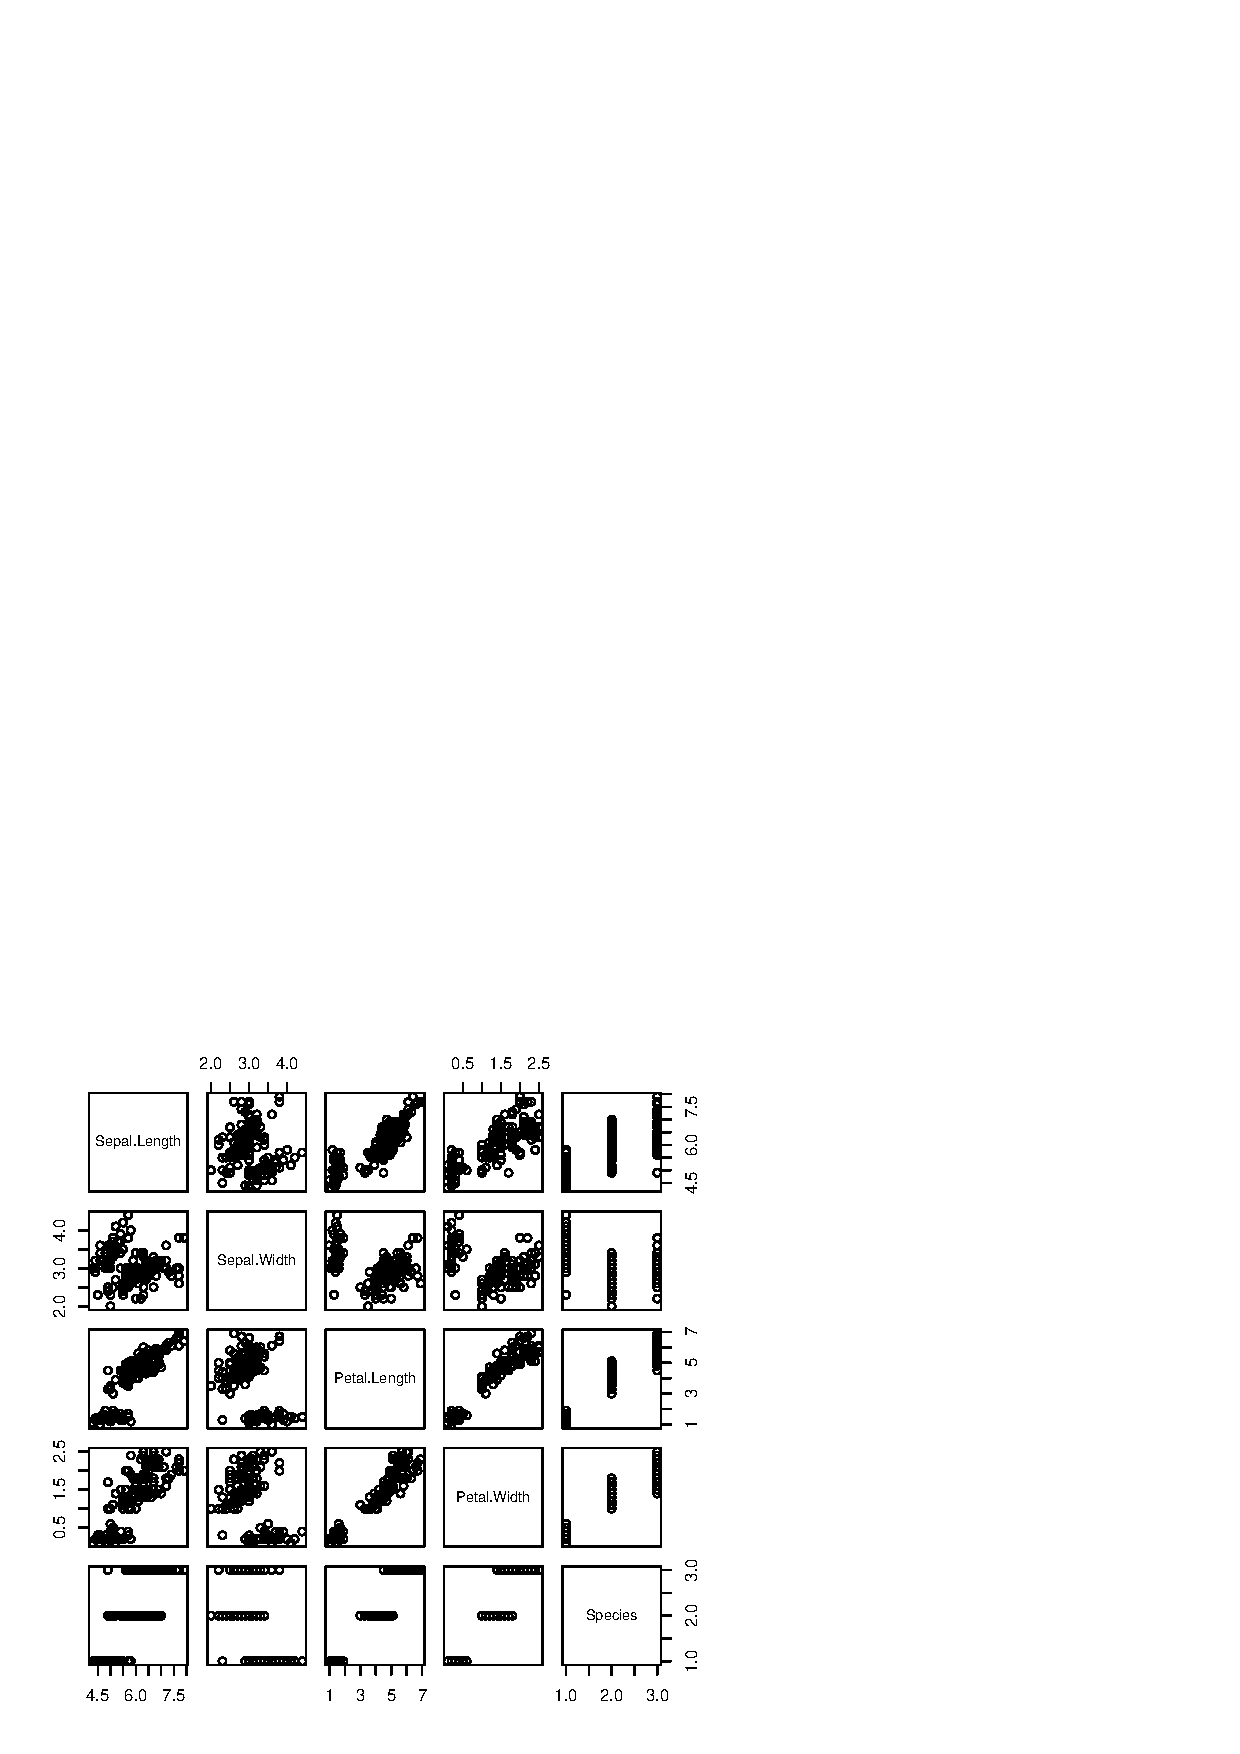
\includegraphics{brew-test-1-1}
    \caption{Pairs plot of the iris data.}
  \end{center}
\end{figure}


\begin{figure}[htbp]
  \begin{center}
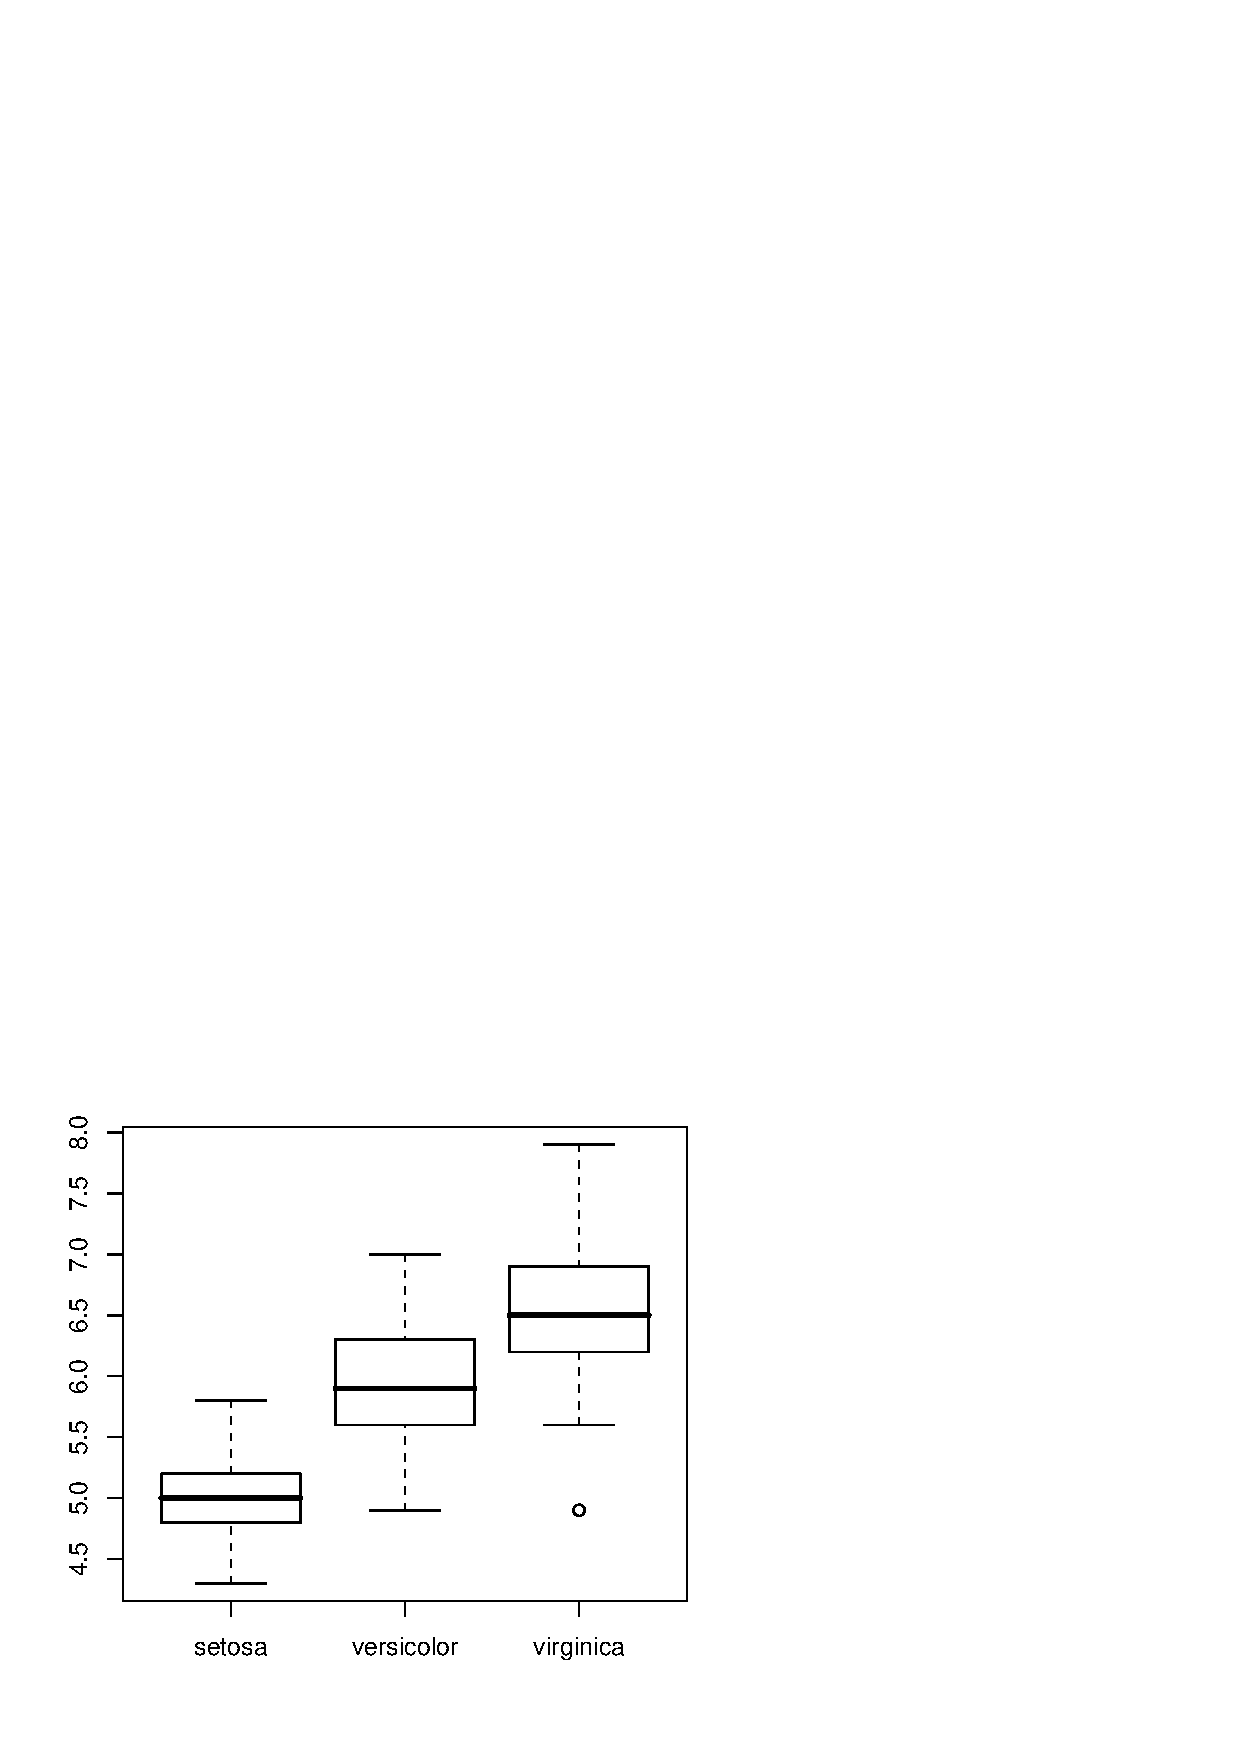
\includegraphics{brew-test-1-2}
    \caption{Boxplot of sepal length grouped by species.}
  \end{center}
\end{figure}

\end{document}


